\chapter{Surrogate Assisted Optimization}
\label{chapter:3}

\begin{tcolorbox}
\textit{The works presented in this chapter have been published in the following articles:}
\begin{enumerate}
\small
\item \textbf{Islam,~M.~M.}, {Singh,~H.~K.},  {Ray,~T.}, and {Sinha,~A.} ``An Enhanced memetic algorithm for single-objective bilevel optimization problems,'' {\em Evolutionary Computation}, MIT press, 2016~\textbf{(Impact factor: 3.6)}.
\item \textbf{Islam,~M.~M.}, {Singh,~H.~K.}, and {Ray,~T.}, ``A Memetic Algorithm for Solving Bilevel Optimization Problems with Multiple Followers,,'' in {\em Proceedings of IEEE Congress on Evolutionary Computation (CEC)}, Vancouver, Canada, pp. 1901--1908, 2016.
\item  \textbf{Islam,~M.~M.}, {Singh, H.K.} and {Ray, T.}``A Memetic Algorithm for the Solution of Single Objective Bilevel Optimization Problems,,'' in {\em Proceedings of IEEE Congress on Evolutionary Computation (CEC)}, Sendai, Japan, pp. 1643-1650, 2015.

\end{enumerate}

\end{tcolorbox}


\section{Introduction}
\label{sec:intro}






\section{Background}
\label{sec:back}

\section{SAMO-IS}

\section{Introduction} Many optimization problems in engineering, finance, operations research and
several other domains have multiple conflicting objectives that need to be minimized/maximized
simultaneously. Population based stochastic algorithms such as Evolutionary algorithms~(EAs) are
commonly preferred for solving such problems as they can deliver a set of non-dominated solutions in
a single run. Furthermore, since EAs do not require assumptions on continuity and differentiability
of the underlying objective and constraint functions, they can be applied to a wide range of
problems. However, being population based methods, EAs require evaluation of numerous solutions
before converging to the set of Pareto optimal solutions. This becomes computationally
prohibitive for problems where evaluation of each candidate solution involves computationally
expensive analysis, such as computational fluid dynamics~(CFD), finite element analysis~(FEA),
computational electromagnetism~(CEM), etc.

Surrogate assisted optimization~(SAO) approaches have long been used for the solution of such
problems, where approximations/surrogates are used in lieu of computationally expensive simulations
during the course of search. Existing SAO approaches use a variety of surrogate models~(global
versus local, single type surrogate versus multiple types) and model management strategies~(periodic
retraining, elite re-evaluation, ranking a mixed bag of individuals, i.e. approximated and truly
evaluated, etc). The choice and effects of surrogate models and model management strategies have
often been matters of discussion, and which method is best is still an issue for
research~\cite{wang_review_2007, jin2005csf}.

In terms of the type of surrogate model, typical models include multi-layer perceptrons, radial
basis function networks, response surfaces of first and second order, Kriging and CoKriging models.
It is difficult to justify the use of one type of surrogate over another. A vast majority of SAO
methods use a single global surrogate model, i.e., one global surrogate for each objective and
constraint function. The surrogate model is either created once and used throughout the course of
search, or created/updated periodically. Algorithms which only build the surrogate
once~\cite{wilson2001epf,goel_ensemble_2007}, rely heavily on the quality of initial samples.
Periodic re-training of the surrogate models is often necessary to capture local behavior of
functions and there are reports on the use of hierarchical surrogate
models~\cite{zhou_combining_2007} to address this. Construction of hierarchical surrogates by space
reduction has also been reported in~\cite{wang_fuzzy_2004}. Hess et al.~\cite{Hess13} suggest to use
machine learning techniques to learn, during the optimization, which surrogate model is most
helpful.

To improve the prediction accuracy with limited samples, multiple surrogates can be used in lieu of
a single surrogate model. Common use of multiple surrogates is in the form of surrogate
\textit{ensembles}, where a collection of surrogate models with varying parameters are usually
trained simultaneously by techniques such as bagging~\cite{breiman_bagging_1996} and
boosting~\cite{abney_boosting_1999}. There are also reports on the use of best local
surrogates~\cite{isaacs2009multi} and the use of multiple approximation models for local
search~\cite{zhou_memetic_2007}. Aggregation and weighted aggregation principles appear to be the
most common strategies to deal with multiple
surrogates~\cite{goel_ensemble_2007,zerpa_optimization_2005, hamza2012co}, and have been used in
both single objective optimization~\cite{glaz2009rotor} and multiobjective
optimization~\cite{mack2005bluff}. There are also reports on the use of the best global surrogate
model for single objective design optimization of turbines~\cite{goel2006perf}. 
While the merit of a surrogate is often judged using the mean squared error~(MSE), there are suggestions 
on the use of correlation measures\cite{shi2008corr}. 

In the context of multiobjective optimization, a multi-layer perceptron was periodically re-trained
and used in alternation with the actual evaluations to solve a B-spline curve fitting problem
in~\cite{nain_computationally_2002}. A similar approach of alternating between actual analysis and
surrogate models has also been reported in~\cite{ray2006sae}.

From the above discussion one can summarize the observations as follows: 
\begin{enumerate} 
	\item
	Various types of surrogates have been used in SAO. Most of them use a single type of surrogate to
	approximate all the objectives and constraint functions. 
	\item In most applications, there is little rationale provided to
	justify the selection of a particular type of surrogate over another. In absence of such an information,
	the choice can only be attributed to user familiarity with the type of surrogate model.
	\item It can
	be further argued that the objectives and constraint functions are likely to have different levels
	of non-linearity. Thus a \textit{single type fits all} strategy may not be the best approach. 
	\item
	Furthermore, in any SAO, the search is likely to intensify in different regions of the search space
	over time. This implies that the most appropriate surrogate for even a single function might vary
	over time, i.e., the best surrogate for an objective might be of different type in different regions
	of the search space. 
	\item Ranking a mixed bag of solutions i.e. a mix of approximated solutions
	and truly evaluated solutions together is a strategy that needs careful attention. Ranking a mixed bag of  solutions 
	require accurate surrogates i.e. ones which have low MSE~(not high correlation coefficient).
\end{enumerate}

This paper is an attempt to address the above issues. A framework for surrogate assisted
multiobjective optimization is introduced, where multiple~\emph{local} surrogates are employed to
approximate the objective and constraint function(s). The approach chooses the best~\textit{local}
surrogate among Kriging, Radial basis function~(RBF), Polynomial response surface method~(RSM) of
order 1 and 2 and Multilayer perceptrons~(MLP) for each objective and constraint function based on mean squared error~(MSE) of the validation set. Since all
possible surrogate models are trained for each objective and constraint function, the flexibility of
representation is not limited as in single type of surrogate based approaches~(both local and
global). Furthermore, local surrogates offer the possibility of better representation that may be
required in later stages of search. While training all possible surrogates for all functions comes
with a computational cost higher than single global surrogate models, the cost of training is
considered insignificant when compared with true evaluations in our current context.

A multiobjective EA is used to search around each generated offspring solution using the best local
surrogate for each objective and constraint function. The final population of all such individual runs are accumulated in an offspring pool.
Our intent is to evaluate $P$ offspring solutions from the accumulated pool in each generation. We adopt two pre-selection strategies i.e. (a)
best $P$ offspring solutions are evaluated using the actual analysis and (b) the offspring pool is combined with existing parents and the best $P$ offspring solutions are evaluated.
Note that as Figure~\ref{fig:selectiondiff} shows, the presence or absence of a parent individual during the
selection step can change the relative ranking among the offspring solutions in a multiobjective setting, which remains unaffected in a single objective setting.

\begin{figure}[!htb] \centering
	\subfloat[]{\label{fig:SAMO_IS}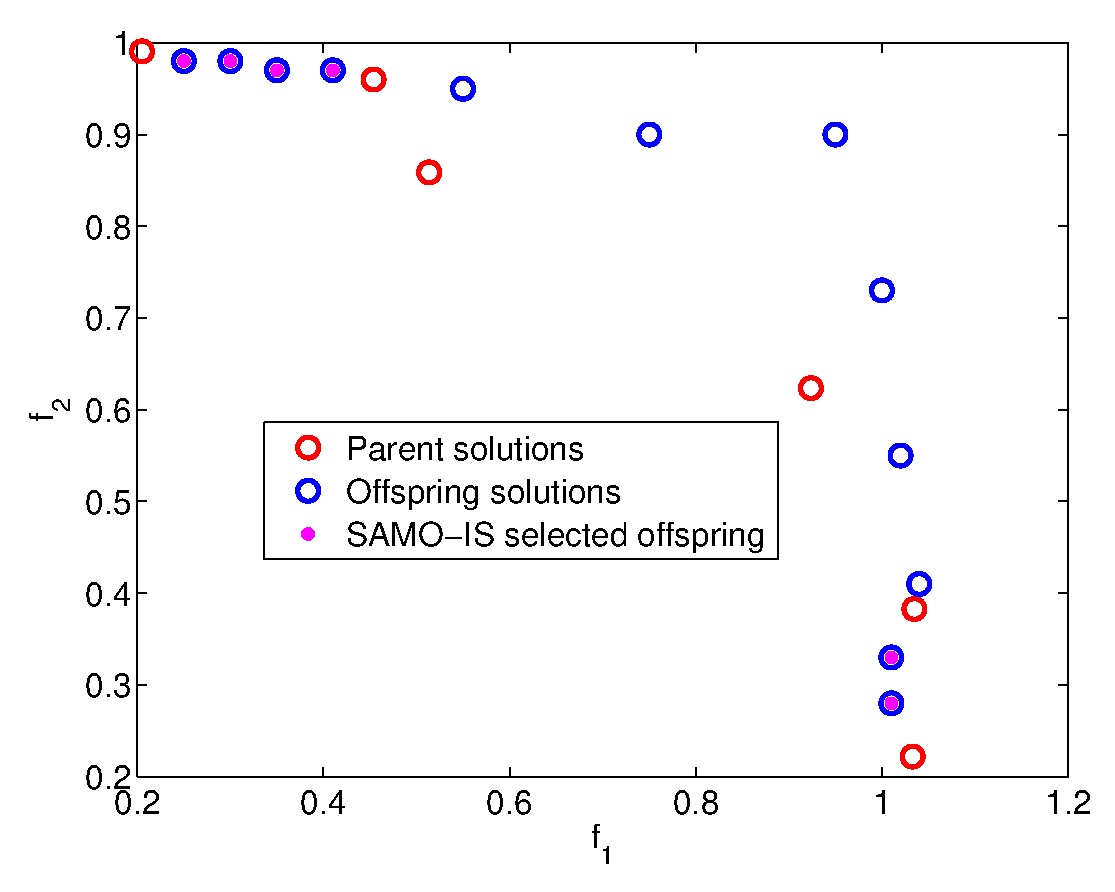
\includegraphics[width=.47\linewidth]{Figures/SAMO_ISselection.eps}}
	\subfloat[]{\label{fig:SAMO}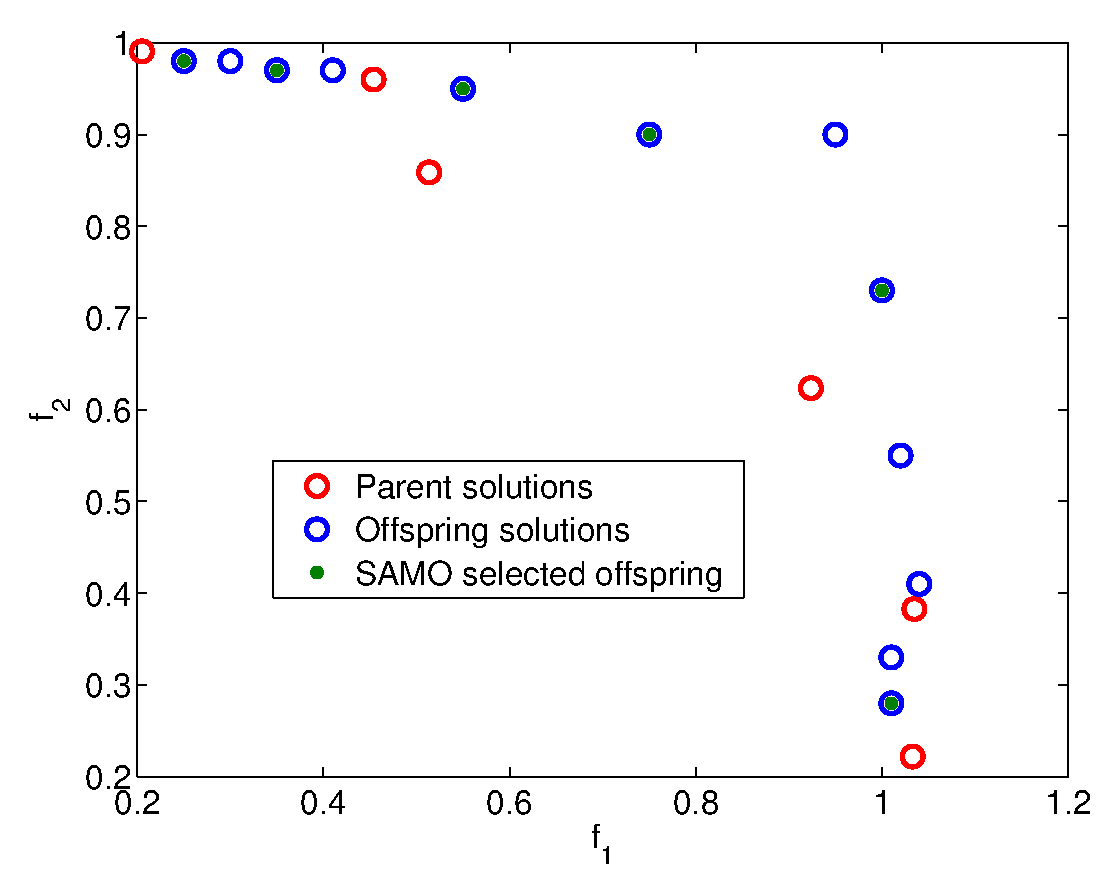
\includegraphics[width=.47\linewidth]{Figures/SAMOselection.eps}}
	\caption{Selection: (a) SAMO-IS (b) SAMO} \label{fig:selectiondiff} \end{figure}

Overall, five strategies have been studied in the paper and all of them have been implemented within
a common framework. These are: 

\begin{enumerate} 
	\item Surrogate
	Assisted multiobjective~(SAMO) algorithm, where multiple local surrogate models are used to
	pre-select most promising offspring solutions without considering parents into account. 
	\item SAMO with
	Improved Selection~(SAMO-IS) where multiple where multiple local surrogate models are used to
	pre-select most promising offspring solutions while considering information of the parents 
	\item SAMO using global model~(SAMO\textsubscript{G}). i.e. one which uses a single global surrogate for each objective
	and constraint function \item SAMO\textsubscript{G} with improved
	selection~(SAMO\textsubscript{G}-IS) i.e. one which uses a single global surrogate model for each objective
	and constraint function and considers information of the parents during pre-selection 
	\item Lastly, 
	we also compare all above strategies the base algorithm~(NSGA-II) which does not use any surrogates. 
\end{enumerate}

\section{Surrogate Assisted multiobjective Optimization} \label{sec:algo} The pseudo-code of the
proposed algorithm is presented in Algorithm~\ref{alg:SAMO}. SAMO relies on
NSGA-II~\cite{deb2002fae} as its baseline EA i.e. the basic operators for parent selection,
recombination and environmental selection are the same. However, SAMO employs a different process to
generate a large pool of offspring solutions and also employs a different selection scheme to
identify promising offspring solutions for evaluation. The principles are explained in the context of minimization. 

\begin{algorithm}[!ht]\footnotesize 
	\caption{SAMO, SAMO-IS} 
	\begin{algorithmic}[1] 
		\REQUIRE
		$TFE_{max}$\qquad \COMMENT{Maximum number of overall actual function evaluations}\\ 
		\REQUIRE $n$\qquad
		\COMMENT{Number of variables of the problem}\\ 
		\REQUIRE {$|P^j| \ge 2\times(n+1)$\qquad 
			\COMMENT{Population
				size}}\\ 
			\STATE $TFE$ = 0, $j$ = 1 \STATE Set archive $\mathcal{A} = \emptyset$ \qquad
		\COMMENT{Archive of all truly evaluated solutions}\\ \STATE $P^j$ = \textbf{Initialize}(),
		$\left|P^j\right| \ge 2\times(n+1)$ \STATE \textbf{Evaluate}($P^j$), Update($TFE$) \STATE
		\textbf{Rank}($P^j$) \STATE Add $P^j$ to archive~($\mathcal{A}$)
		
		\WHILE{{$(TFE < TFE_{max})$}} \STATE $C$ = \textbf{CreateOffspring}($P^j$), $\left|C\right|$ =
		$\left|P^j\right|$ \STATE $n\_neighbor$ = $\min$($\left|\mathcal{A}\right|$, 4$\times n$) \STATE
		$C_s$ = $C$ - ($C \cap \mathcal{A}$)\qquad \COMMENT{Unique solutions with respect to Archive}\\
		\STATE $C_{NDset}$ = $\emptyset$ \FOR{$i = 1:\left|C_s\right|$} \STATE
		[$\mathcal{N}_{{C^{i}}_s}$,$\mathbb{R}_{{C^{i}}_s}$] =
		\textbf{SetRangeNeighbor}(${C^{i}}_s$,$\mathcal{A}$,$n\_neighbor$) \STATE $\mathcal{S}_{{C^{i}}_s}$
		= \textbf{BuildSurrogate}($\mathcal{N}_{{C^{i}}_s}$,$\mathbb{R}_{{C^{i}}_s}$) \STATE $C_{ND}$ =
		\textbf{RunEA}($\mathcal{S}_{{C^{i}}_s}$,$\mathbb{R}_{{C^{i}}_s}$)\\ \STATE Append $C_{ND}$ to
		$C_{NDset}$ \ENDFOR \STATE $C_{NDpool}$ = $P^j \cup C_{NDset}$\qquad \COMMENT{Actually evaluated
			parents are combined with the offspring set}\\ \STATE $C^j$ =
		\textbf{GetoffspringEval}($C_{NDpool}$) $|$ $\left|C^j\right|$ =
		$\min$($\left|P^j\right|$,$\left|C_{NDset}\right|$)\\ \STATE $C^j$ = $C^j$ - ($C^j \cap
		\mathcal{A}$)\qquad \COMMENT{Unique solutions with respect to Archive}\\ {\IF{$|C^j| > TFE_{max} - TFE$}
			\STATE Choose top $C^j$, $|C^j| = TFE_{max} - TFE$ \ENDIF} \STATE \textbf{Evaluate}($C^j$), Update($TFE$) \STATE Add $C^j$ to archive~($\mathcal{A}$) \STATE
		\textbf{Rank}($P^j + C^j$) \STATE $P^{j+1} = $\textbf{Reduce}($P^j + C^j$) \STATE $j$ = $j$ + 1
		\ENDWHILE
		
	\end{algorithmic} 
\label{alg:SAMO} 
\end{algorithm}

The highlighted parts of the algorithm are explained below:\\ 
\begin{enumerate} 
	\item
	\textbf{Initialize}: The solutions of the population are initialized using Latin Hypercube
	Sampling~(LHS). The size of the population should be even and $\geq 2(n+1)$.
	\item \textbf{Evaluate}: Objective and constraint function values are computed for
	all the solutions using actual evaluations. \item \textbf{Rank}: Ranking of the solutions follows
	the \textit{feasibility first} principle. The feasible solutions are sorted based on non-domination
	rank and crowding distance. The infeasible solutions are ranked based on the sum of constraint
	violations. 
	\item \textbf{CreateOffspring}: This process involves generation of a set of offspring
	solutions via binary tournament, simulated binary crossover and polynomial
	mutation~\cite{deb2002fae}. \item \textbf{SetRangeNeighbor}: For each offspring solution in $C_s$,
	$n\_neighbor$ number of neighboring solutions~($\mathcal{N}_{{C^{i}}_s}$) are identified from the
	archive $\mathcal{A}$ based on the distance computed in the normalized variable space. The bounds
	for this set of neighboring solutions are $\mathbb{R}_{{C^{i}}_s}$(lower) = $\min_{\forall (1\dots
		n)} \mathcal{N}_{{C^{i}}_s}$ and $\mathbb{R}_{{C^{i}}_s}$(upper) = $\max_{\forall (1\dots n)}
	\mathcal{N}_{{C^{i}}_s}$. The maximum number of neighbors is set to $4 \times n$. This is only used
	when local surrogates are used for approximation. 
	\item \textbf{BuildSurrogate}: This process
	involves building the surrogate models for each constraint and objective function separately using
	different types of approximation methods: Radial Basis Function~(RBF), Kriging, Multi-layer
	Perceptron~(MLP), Response Surface Methodology~(RSM) of $1^{st}$ and $2^{nd}$ order. For each
	offspring solution~(${C^{i}}_s$), the above surrogate models are constructed for each objective and
	constraint function. A fraction of solutions from the archive~(neighbor set for local surrogates)
	are used to train the surrogate models, while the rest are used for validation. Mean squared
	error~(MSE) based on the validation set is used to choose the most appropriate surrogate for each
	constraint and objective function. Since the pool of offspring solutions  are ranked~(among themselves in SAMO and along with all solutions evaluated using actual analysis in SAMO-IS), 
	the surrogates need to be assessed based on MSE. It is also important to take note that such surrogates are only used
	within the limits of the variable bounds of the neighbor set used for local surrogates, while the
	overall variable bounds are used for global surrogates. 
	\item \textbf{RunEA}: For each offspring
	solution, a population of 100 individuals is initialized using the bounds as discussed above and
	evolved over 20 generations using the best surrogate for each constraint and objective function
	resulting in a set of non-dominated solutions~($C_{ND}$). \item \textbf{GetOffspringEval}: This 
	stage involves selecting top unique non-dominated offspring solutions from the combined set 
	of solutions obtained from the above step~($C_{NDpool}$). $C_{NDpool}$ is essentially a union of 
	all the non-dominated offspring solutions obtained from NSGA-II runs. In SAMO-IS, top unique non-dominated 
	offspring solutions from the combined set of solutions ~($C_{NDpool}$) and all truly evaluated parents 
	undergo evaluation. The differences in SAMO-IS and SAMO selection is 
	illustrated using Figure~\ref{fig:selectiondiff}. Since SAMO-IS uses information of the parents, it will ignore 
	evaluation of offspring solutions if they are dominated by the parents and thus will have a greater selection
	pressure as compared to SAMO.
	\item
	\textbf{Reduce}: The reduction procedure selects the top $\left|P^j\right|$ ranked solutions~(based
	on feasibility first ranking scheme) from the combined set~($P^j + C^j$). \end{enumerate}

To demonstrate the benefits of the proposed approach, its performance against the variants are
studied using four numerical benchmarks~(ZDT1, OSY, SRN, and Test\_Tan), and three engineering
design examples~(Welded beam, Car crash and Bulk carrier design).

\section{Numerical Experiments} \label{sec:results} The numerical experiments are detailed in this
section. We start with a brief recap of the performance metrics, followed by description of the
problems studied and discussion of relative performance of various strategies.

\subsection{Performance Metrics}

\subsubsection{Hypervolume} The qualitative performance of any multiobjective optimization
algorithm can be qualitatively deduced from visualizing the non-dominated front. For an objective
comparison, quantitative measures are required for convergence and diversity. One such measure is
Hypervolume~(HV) introduced by~\cite{zitzler1999multiobjective}. It measures the the volume of the
dominated portion of the objective space with respect to a reference point. Given a set of nondominated solutions and their corresponding objective vectors, we first discard all solutions that lie outside the hyper-box constructed using \{$0,0,\dots,0$\} and the Nadir vectors listed in Table \ref{tab:hvstat1} and Table \ref{tab:hvstat2}. The objective vectors of the remaining solutions are normalized using the \{$0,0,\dots,0$\} and the Nadir vector. The HV is subsequently computed with the reference point as \{$1.1,1.1,\dots,1.1$\}. 

\subsubsection{Performance profiles} Apart from reporting performance on individual problems using hypervolume metric, performance
profile proposed in \cite{dolan2002perf} is also used to compare different algorithms based on the overall performance in all the problems. In a plot of performance profile, the horizontal
axis~($\tau$) signifies the performance values within a threshold value for each problem. The
vertical axis~($\rho(\tau)$) signifies the cumulative distribution of the performance. Since a
higher HV is better, inverse of median hypervolume values~(delivered by all the algorithms across
all problems) have been used in this study to be consistent with the notion of performance profile
plots. Area under the performance profile curve~($AUC = \int{\rho(\tau)d\tau}$) represents the overall
performance of any algorithm over the problem set in consideration. The larger the $AUC$, the higher
is the efficiency of the algorithm. By convention, performance profiles consider a lower value of given metric to be better~(e.g. time to taken to solve a problem). Hence, in this paper,  in order to follow the convention, inverse of median hypervolume values are considered for the performance profile computation.

\subsection{Experimental set-up and results} In the following numerical examples, the probability of
crossover and mutation are set to 0.9 and 0.1 respectively. The distribution index~(spread of the offspring solution) for crossover is
set to 10 and distribution index for mutation is set to 20. To build the local surrogates, 80\% of
the solutions are used for training and the rest for validation. A maximum of 1000 solutions are
used for training the surrogates. The surrogate delivering the minimum MSE on the validation set is
considered the best for each objective and constraint function. The statistics reported are based on
10 independent runs. It is important to take note that the nondominated set of solutions and
hypervolume computation are based on \textit{all solutions fully evaluated during the run}~(and not
just the final population). This makes sense in SAO, since the assumption is that a full evaluation
is computationally expensive, and thus only relatively few such such solutions are generated during
the run. The algorithm with the problems are made available for download from \cite{mdolabsamois}.

\subsubsection{ZDT1}

ZDT1 is a scalable, multiobjective benchmark problem introduced in \cite{zitzler2000mo}, with a
convex Pareto optimal front~(POF). A 10-variable version is considered here. A population of 22
solutions was evolved with the maximum number of actual evaluations set to 1200.
Figure~\ref{fig:zdt1_Pf} shows the set of solutions obtained using various strategies. The mean
hypervolume values at various costs are presented in Figure~\ref{fig:zdt1_HV}. It is observed that
all the surrogate assisted strategies deliver comparable results, which are significantly better
than the baseline NSGA-II~(which does not use any form of approximation) especially in early stages
of the search.

\begin{figure*}[!htb] \centering
	\subfloat[]{\label{fig:zdt1_Pf}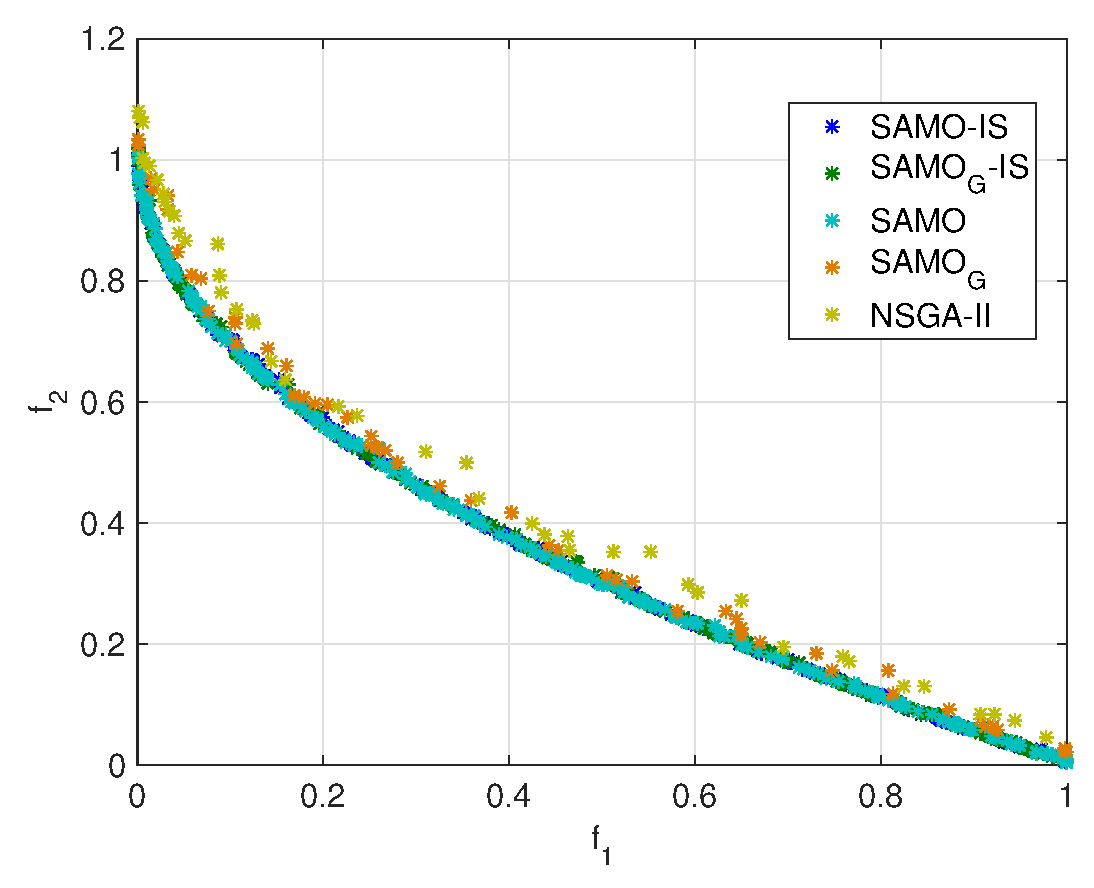
\includegraphics[width=.227\linewidth]{Figures/zdt1_Pareto_median.eps}}
	\subfloat[]{\label{fig:zdt1_HV}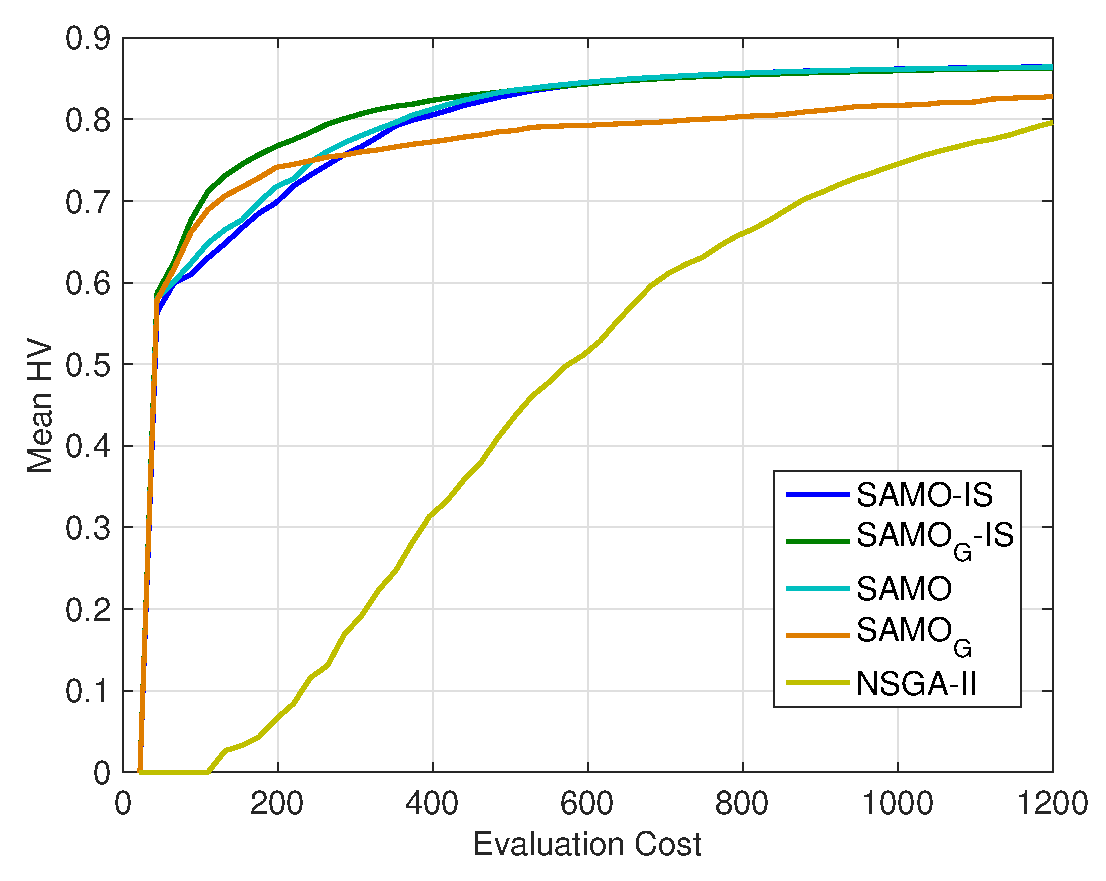
\includegraphics[width=.23\linewidth]{Figures/zdt1_Mean_HV.eps}}
	\subfloat[]{\label{fig:osy_Pf}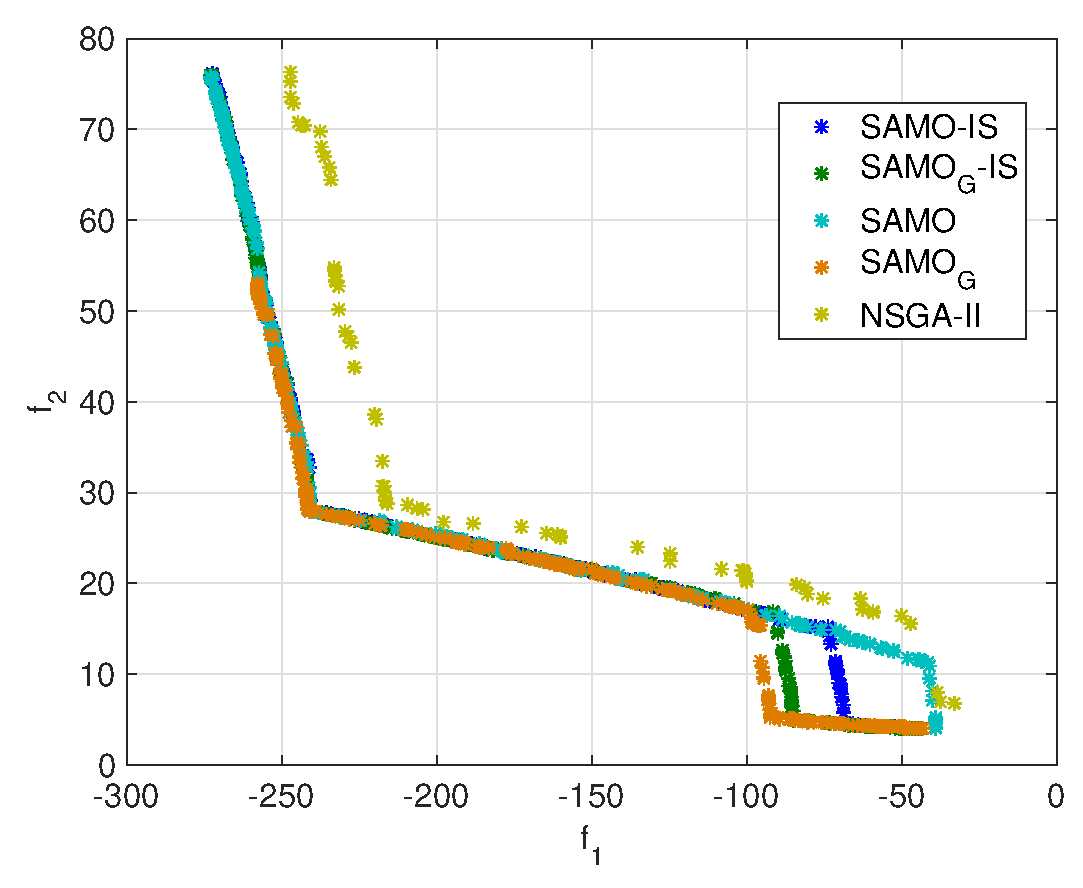
\includegraphics[width=.225\linewidth]{Figures/osy_Pareto_median.eps}}
	\subfloat[]{\label{fig:osy_HV}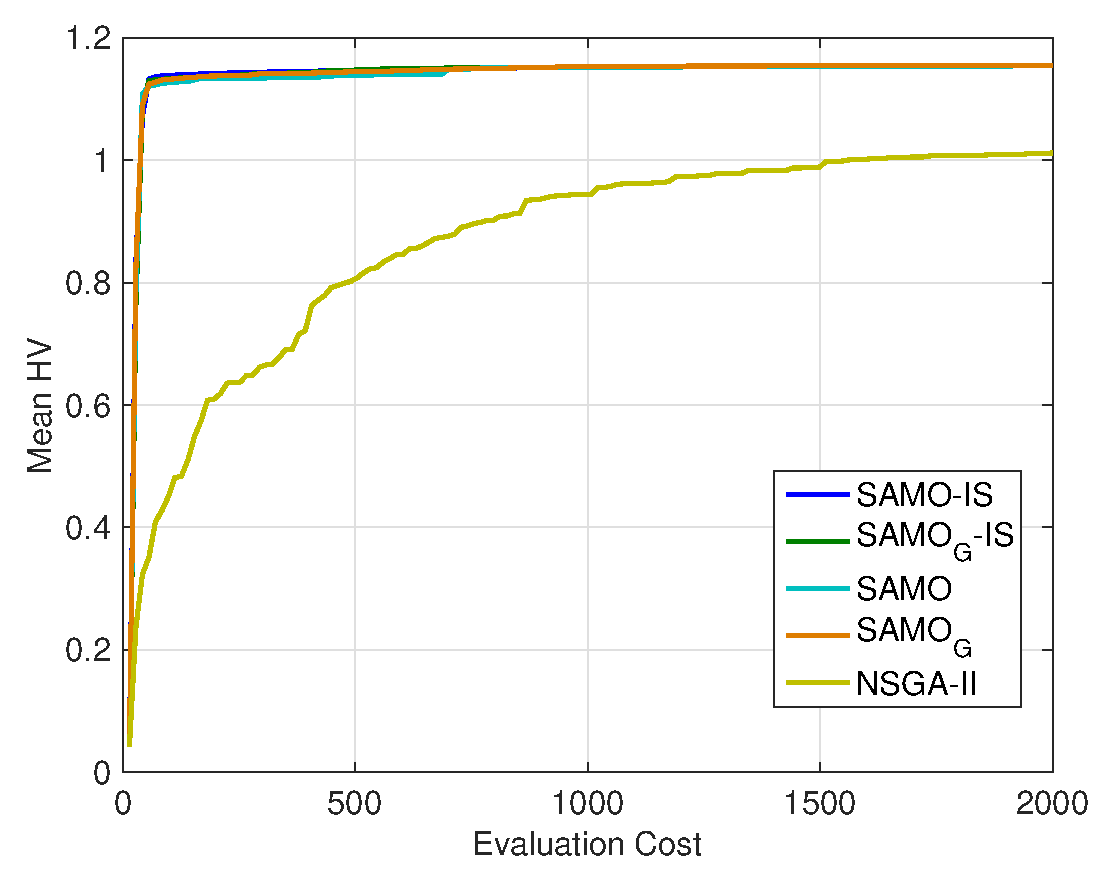
\includegraphics[width=.23\linewidth]{Figures/osy_Mean_HV.eps}}
	\caption{(a) ZDT1: Nondominated front, (b) ZDT1: Mean HV convergence, (c) OSY: Nondominated front, (d) OSY: Mean HV convergence}
	\label{fig:zdt1osy_Pareto} \end{figure*}

\subsubsection{OSY} The OSY problem~\cite{osy1995mc} is a six-variable minimization problem with
two-objectives and six inequality constraints. A population of 22 solutions was evolved with the
maximum number of actual evaluations set to 2000. The mean hypervolume values at various costs are presented in
Figure~\ref{fig:osy_HV}. Once again, all surrogate assisted strategies deliver competitive results
which are significantly better than baseline NSGA-II. One can also observe that the difference in
performance gradually decreases over the course of evolution.

\subsubsection{SRN} The SRN problem~\cite{deb2002fae} is a bi-objective minimization problem with
two-variables and two inequality constraints. A population of 12 solutions was evolved with the
maximum number of actual evaluations set to 1100. The results of all the strategies are presented in
Figure~\ref{fig:srn_Pf} and Figure~\ref{fig:srn_HV}. A similar observation as above can be derived although one can notice
that the gap in performance during the run is relatively small for this problem compared to previous
ones.

\begin{figure*}[!htb] \centering
	\subfloat[]{\label{fig:srn_Pf}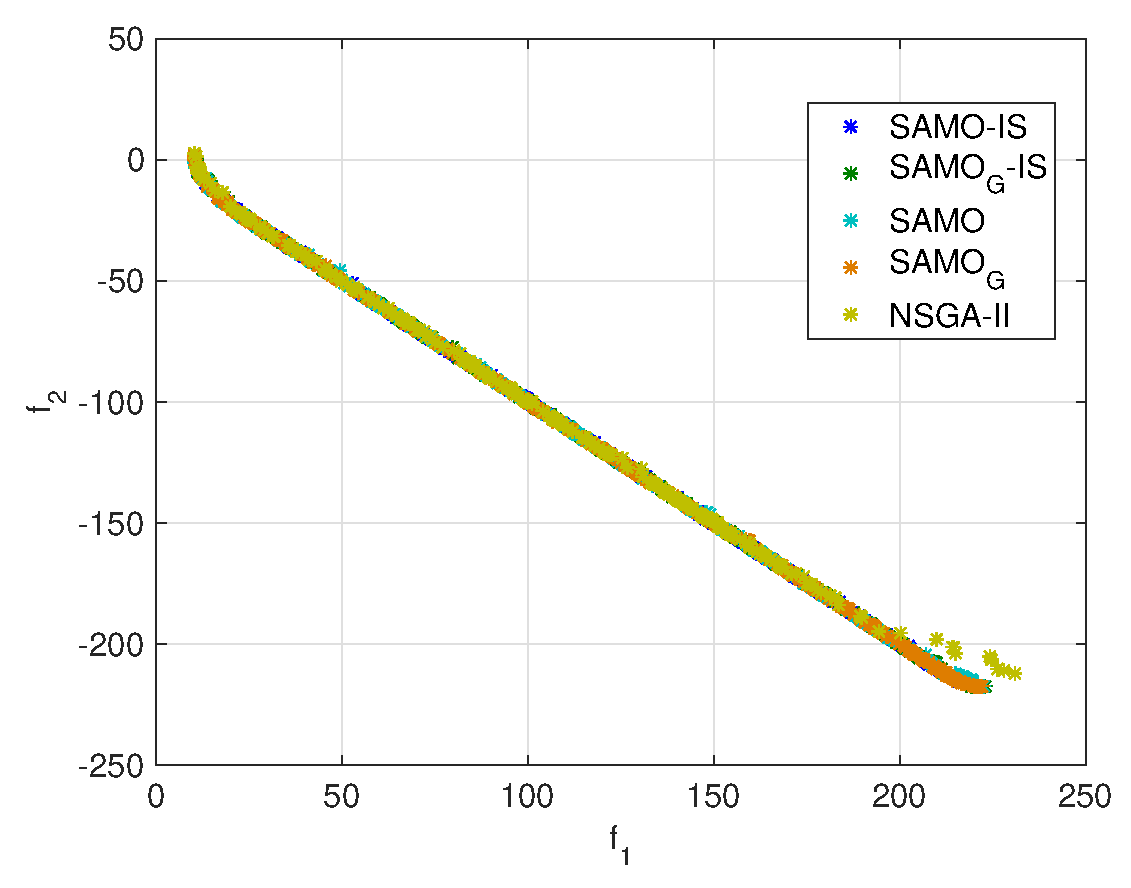
\includegraphics[width=.231\linewidth]{Figures/srn_Pareto_median.eps}}
	\subfloat[]{\label{fig:srn_HV}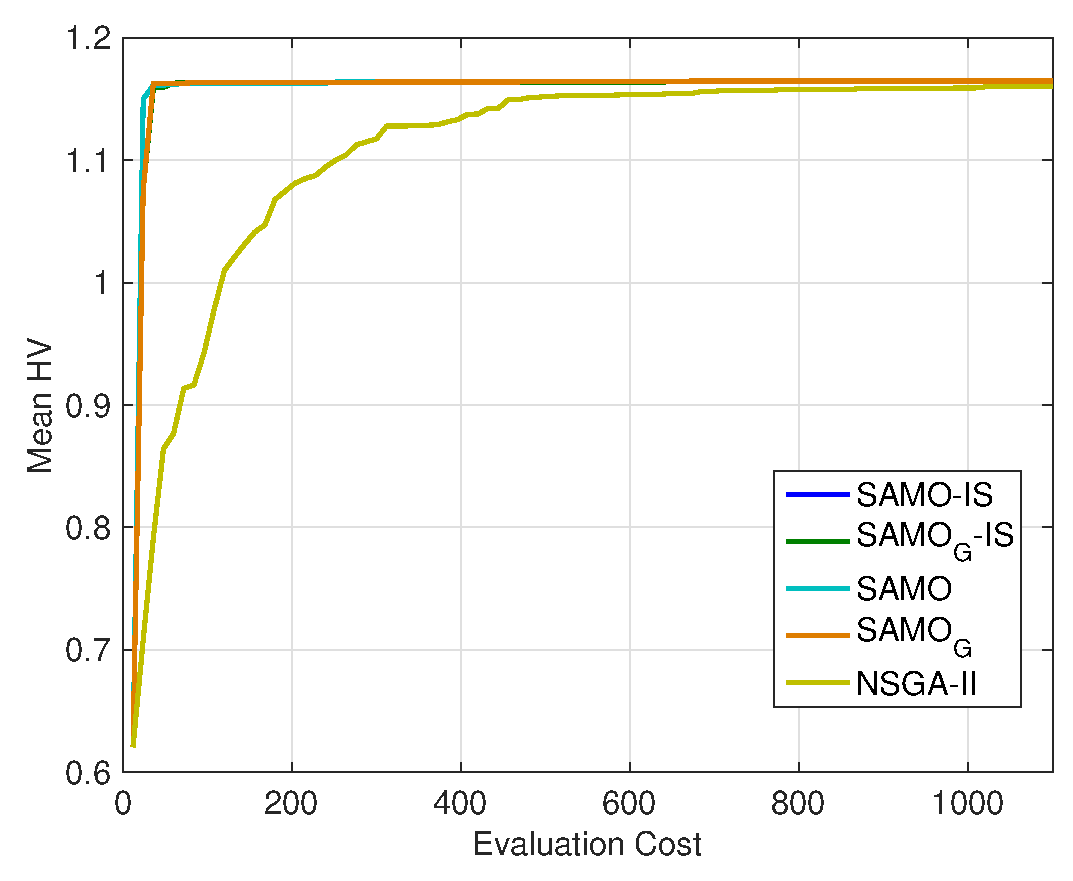
\includegraphics[width=.223\linewidth]{Figures/srn_Mean_HV.eps}}
	\subfloat[]{\label{fig:test_tan_Pf}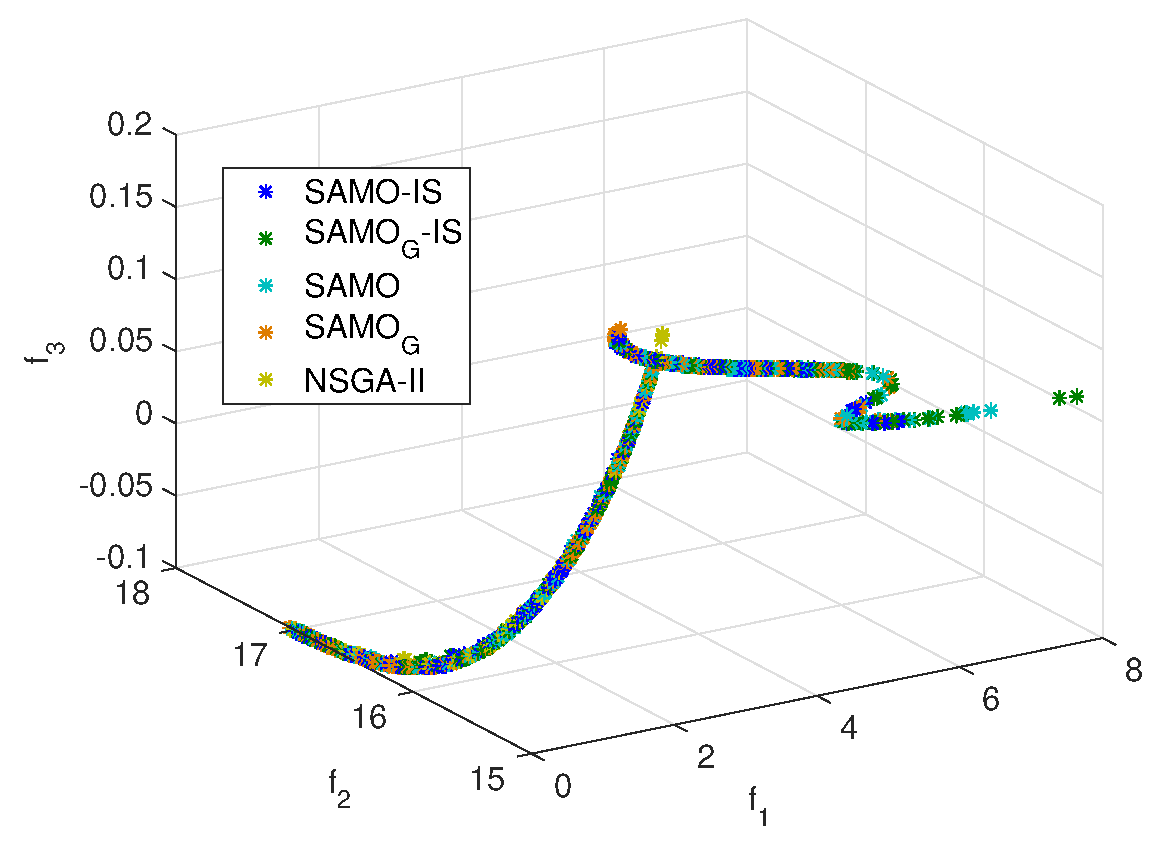
\includegraphics[width=.22\linewidth]{Figures/Test_Tan_Pareto_median.eps}}
	\subfloat[]{\label{fig:test_tan_HV}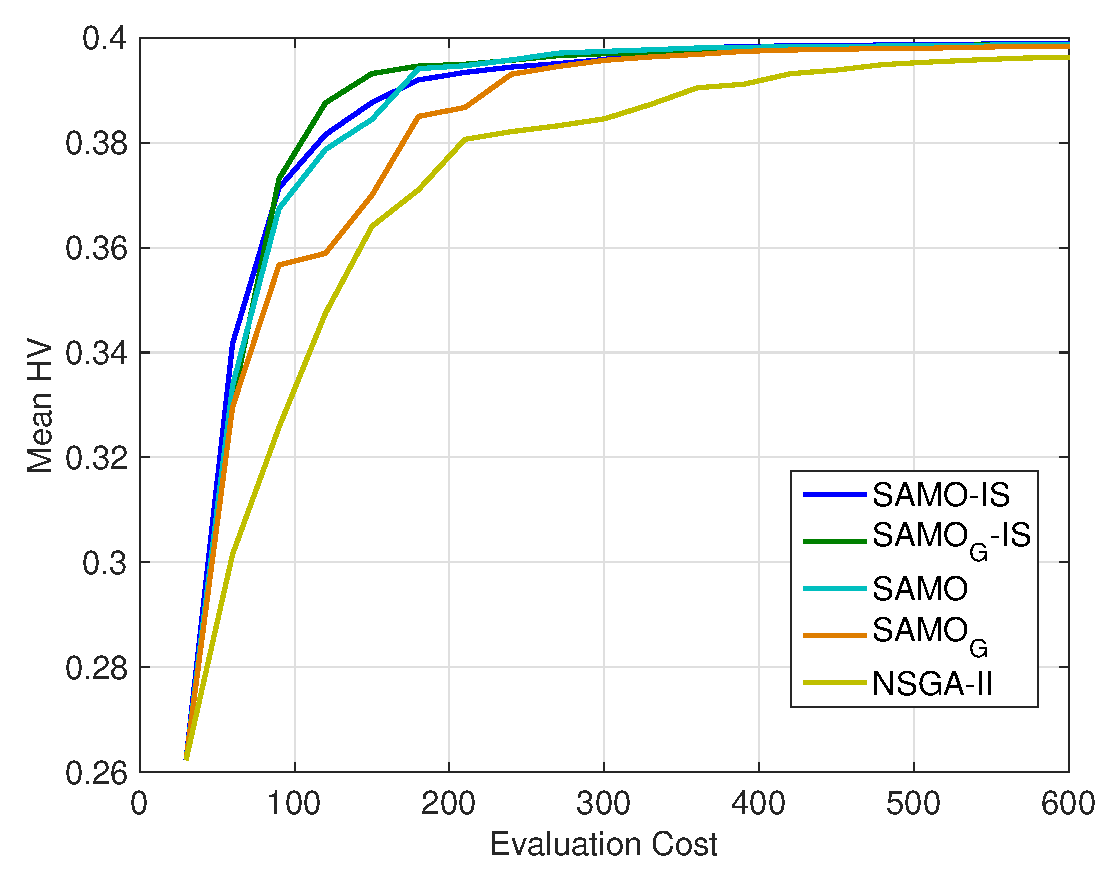
\includegraphics[width=.228\linewidth]{Figures/Test_Tan_Mean_HV.eps}}
	\caption{(a) SRN: Nondominated front, (b) SRN: Mean HV convergence, (c) Test\_Tan: Nondominated front, (d) Test\_Tan: Mean HV convergence} 
	\label{fig:srntesttan_Pareto}
\end{figure*}

\subsubsection{Test\_Tan} The Test\_Tan problem~\cite{Tan2001ec} is a two-variable unconstrained
minimization problem with three-objectives. A population of 30 solutions was evolved with the
maximum number of actual evaluations set to 600. The results of all the strategies are presented in
Figure~\ref{fig:test_tan_Pf} and Figure~\ref{fig:test_tan_HV}. For this problem, one can observe that the rate of convergence of
SAMO\textsubscript{G} and NSGA-II are significantly worse when compared to others.

\subsubsection{Welded Beam} The Welded Beam problem is well studied engineering example presented in
\cite{Deb2000constraint}. The problem involves two objectives and has 4 design variables and 4
inequality constraints. The POF for this problem is of convex nature. For this problem, a population
of 20 solutions were evolved with the maximum number of actual evaluations set to 900. The nondominated solutions obtained at the end of median run using all the strategies are presented in Figure~\ref{fig:welded_beam2_Pf}. It is clear from
Figure~\ref{fig:welded_beam2_HV} that SAMO-IS offers the best solution when compared with others.
Also it is interesting to take note that local surrogates~(SAMO-IS and SAMO) offer better
performance compared to its global counterparts~(SAMO\textsubscript{G}-IS and
SAMO\textsubscript{G}).

\begin{figure*}[!htb] \centering
	\subfloat[]{\label{fig:welded_beam2_Pf}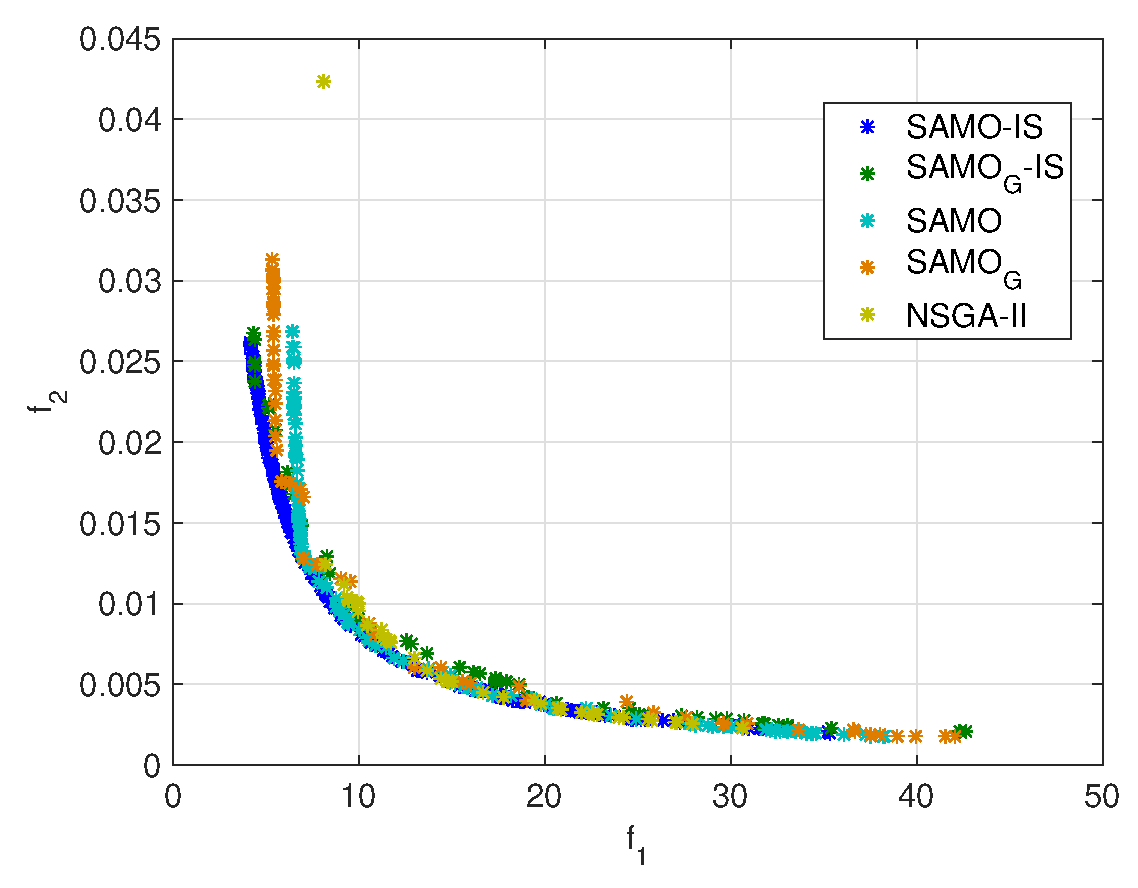
\includegraphics[width=.231\linewidth]{Figures/welded_beam2_Pareto_median.eps}}
	\subfloat[]{\label{fig:welded_beam2_HV}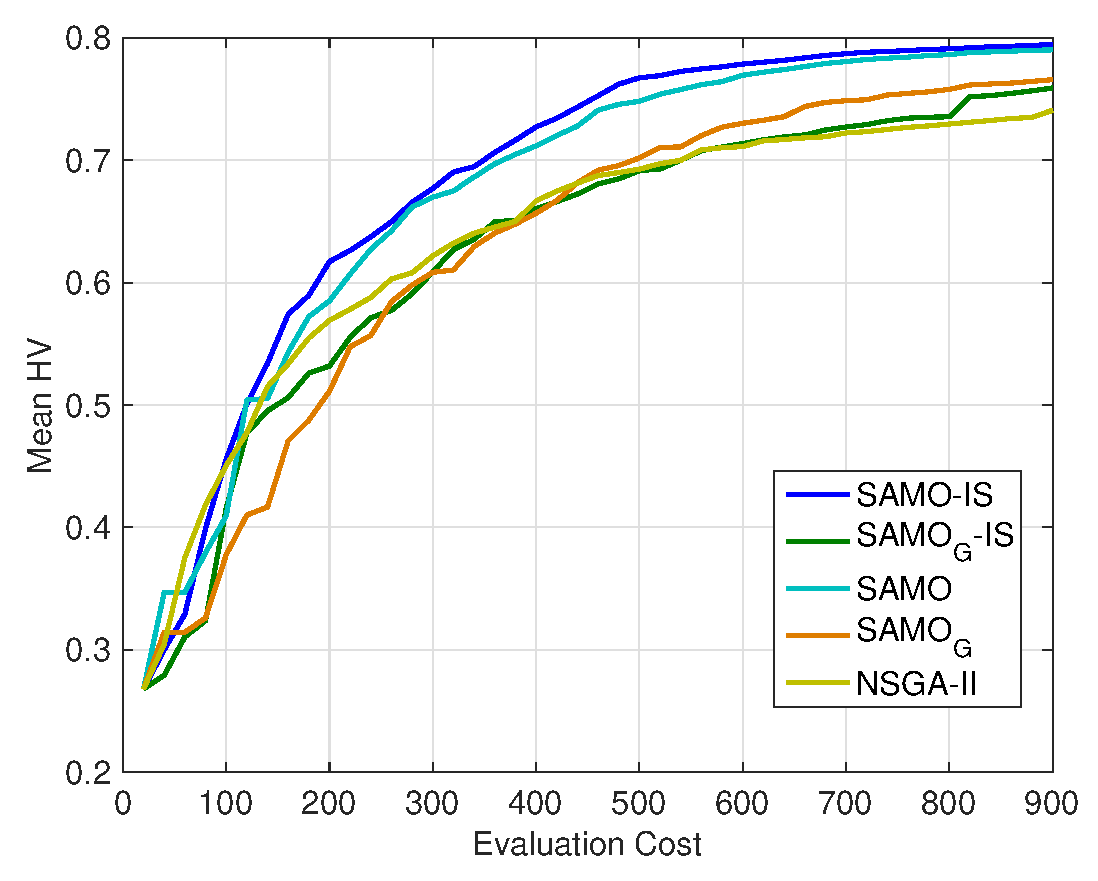
\includegraphics[width=.228\linewidth]{Figures/welded_beam2_Mean_HV.eps}}
	\subfloat[]{\label{fig:Car_Crash_Pf}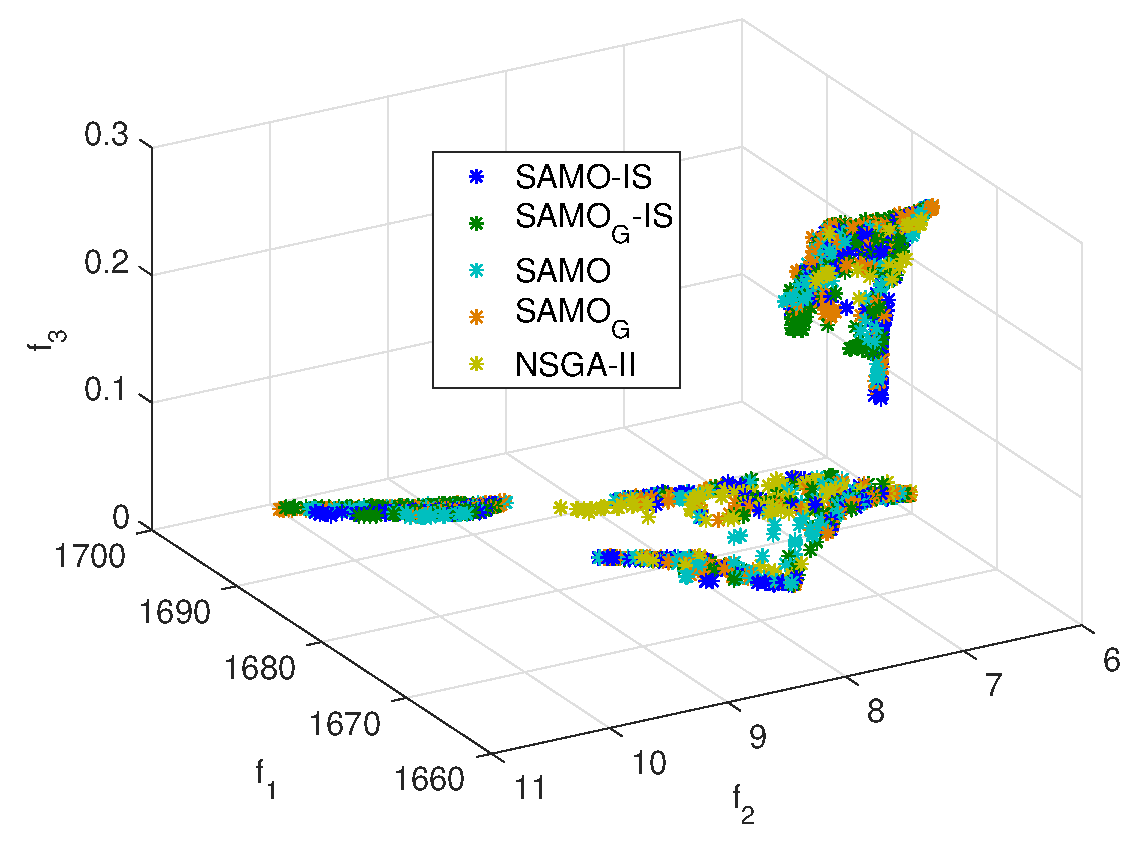
\includegraphics[width=.22\linewidth]{Figures/Car_Crash_Pareto_median.eps}}
	\subfloat[]{\label{fig:Car_Crash_HV}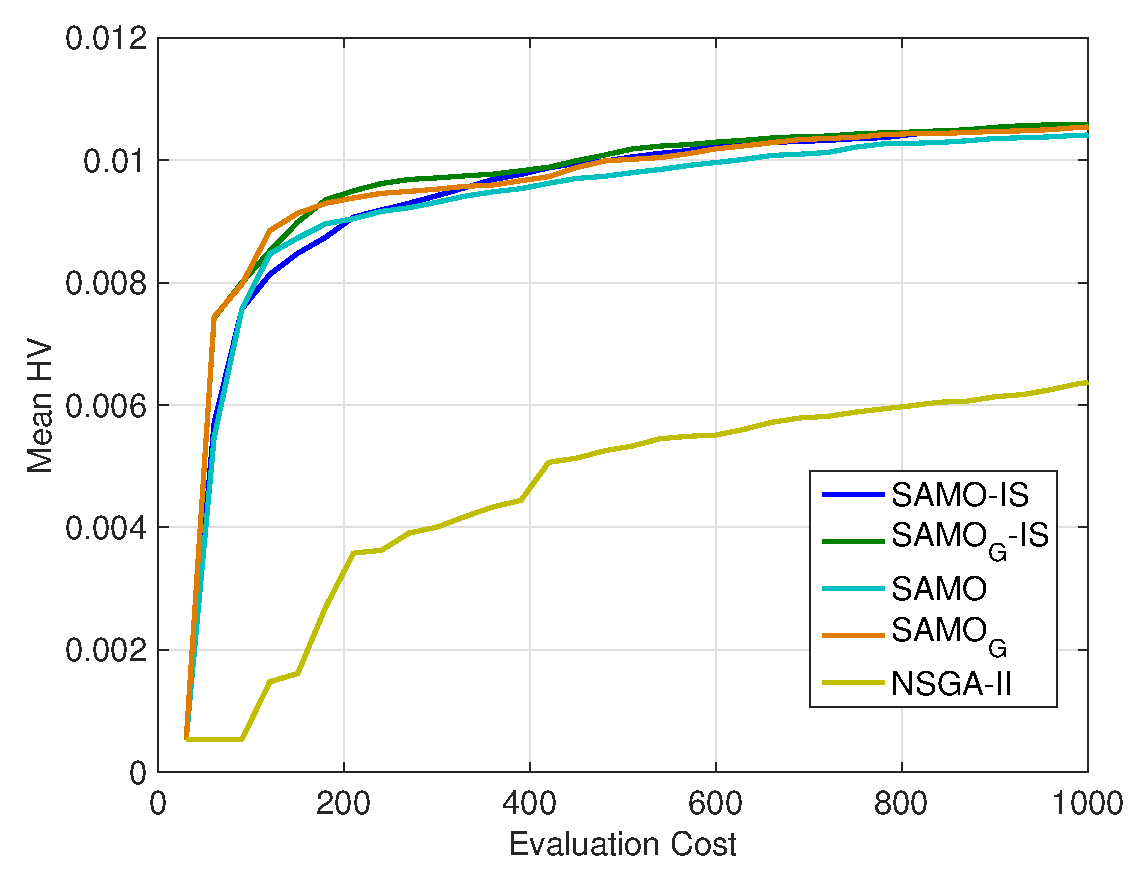
\includegraphics[width=.231\linewidth]{Figures/Car_Crash_Mean_HV.eps}}
	\caption{(a) Welded Beam: Nondominated front, (b) Welded Beam: Mean HV convergence, (c) Car Crash: Nondominated front, (d) Car Crash: Mean HV convergence}
	\label{fig:welded_beam2_Pareto} \end{figure*}

\subsubsection{Car Crash} In this engineering design problem~\cite{Liao2008crash}, there are three
objectives which need to be minimized: mass of the vehicle, integration of collision acceleration
between 0.05s and 0.07s in ``full frontal crash'' and toe board intrusion in
``offset-frontal-crash''. The design variables are the thickness values of 5 reinforced members
around the frontal structure of the vehicle. The POF is reported to be convex, consisting of a set
of disconnected patches. A population of 30 solutions was evolved with the maximum number of actual
evaluations set to 1000. The results using all the approaches are presented in
Figure~\ref{fig:Car_Crash_Pf} and Figure~\ref{fig:Car_Crash_HV}. Based on the mean hypervolume convergence plot, one can observe
that SAMO-IS offers benefits over SAMO, while the results of other surrogate assisted strategies are
quite similar.

\subsubsection{Bulk Carrier Design} The problem was originally introduced in ~\cite{sen1998mcd} and
since then modified in~\cite{augusto2012new}. The problem contains are three objectives:
minimization of lightweight of the ship, maximization of annual transport cargo capacity and
minimization of annual transportation cost. There are 6 design variables: length, breadth, depth,
draft, block coefficient and speed of the ship. There are 9 inequality constraints in the problem,
which relate to length-breadth ratio, length-depth ratio, length-draft ratio, maximum and minimum
allowable draft, hydrostatic stability condition, maximum and minimum allowable deadweight and
Froude number. A population of 28 solutions was evolved with the maximum number of actual
evaluations set to 2000. The results of all the approaches are presented in
Figure~\ref{fig:bulk_carrier_design_Pareto}. One can observe from
Figure~\ref{fig:bulk_carrier_design_HV} that local surrogates~(SAMO-IS and SAMO) offer better
solutions when compared with their global counterparts.

\begin{figure}[!htb] \centering
	\subfloat[]{\label{fig:bulk_carrier_design_Pf}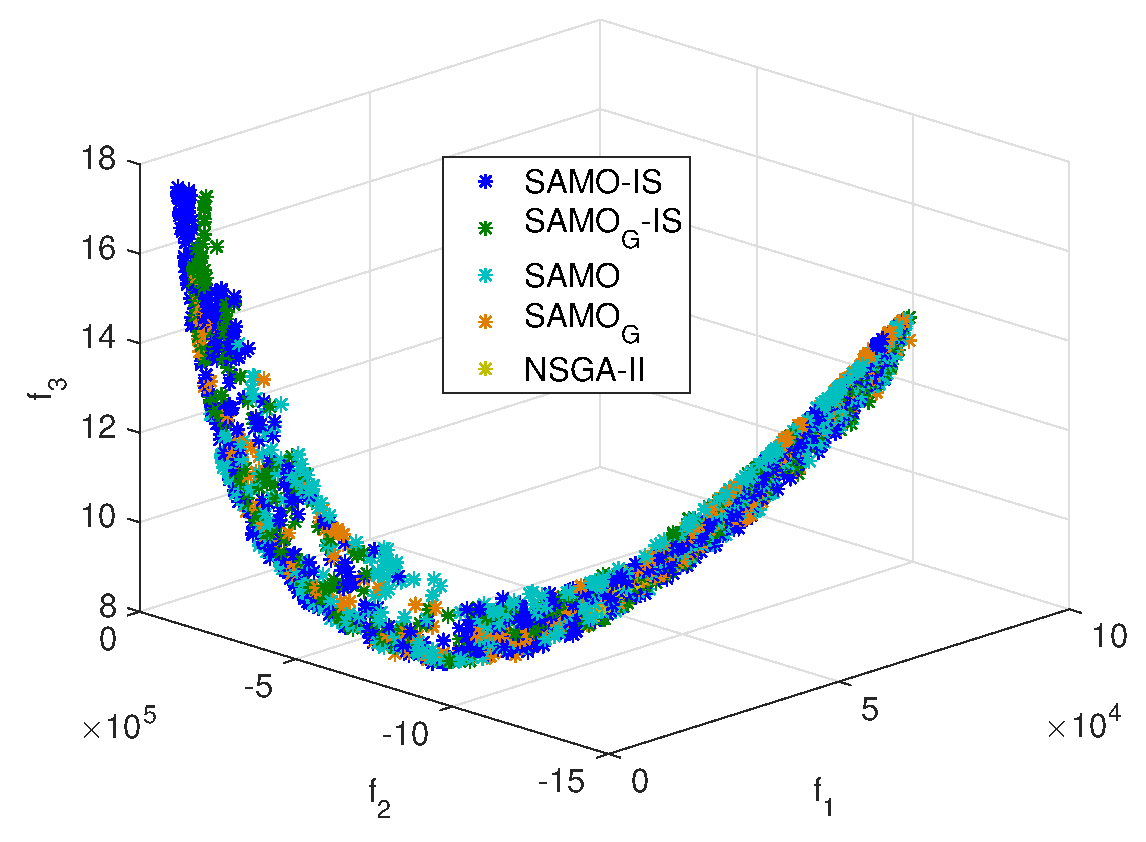
\includegraphics[width=.45\linewidth]{Figures/bulk_carrier_design_Pareto_median.eps}}
	\subfloat[]{\label{fig:bulk_carrier_design_HV}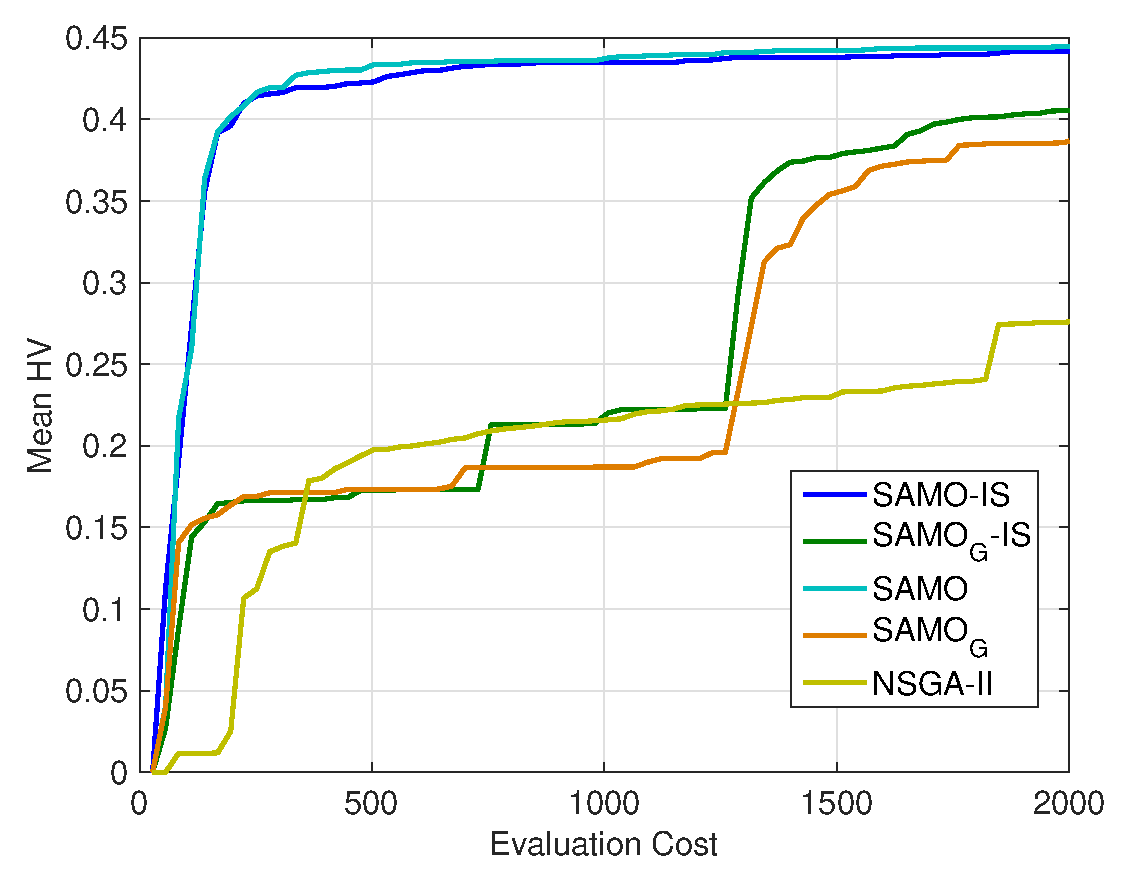
\includegraphics[width=.45\linewidth]{Figures/bulk_carrier_design_Mean_HV.eps}}
	\caption{Bulk Carrier Design: (a) Nondominated front, (b) Mean HV convergence}
	\label{fig:bulk_carrier_design_Pareto} \end{figure}

\subsection{Performance Comparison} HV values presented in the plots earlier are based on mean HVs
across multiple runs. Again, the HV values reported in Table~\ref{tab:hvstat1} and
Table~\ref{tab:hvstat2} and presented in all HV plots are based on all fully evaluated solutions.
The reference points used for HV computation are also listed in the tables. Best median HV values are marked in bold.

\begin{table*}[!ht]\scriptsize 
	\centering 
	\caption{Hypervolume Statistics: Bi-objective problems}
	\begin{tabular}{|l|l|l|l|l|l|l|l|} 
		\noalign{\smallskip}\hline 
		\textbf{Problems} & \textbf{Reference point} & \textbf{Algorithm} & \textbf{Best} & \textbf{Mean} & \textbf{Median} & \textbf{Worst} & \textbf{Std Error} \\ \hline 
		\multirow{5}{*}{\textbf{ZDT1}} & & SAMO-IS & 0.862551 & 0.864638 & \textbf{0.864719} & 0.866242 & 0.000373 \\ 
		& & SAMO\textsubscript{G}-IS & 0.858749 & 0.862596 & 0.863350 & 0.864649 & 0.000671 \\ 
		& [1,1] & SAMO & 0.860722 & 0.864234 & 0.864699 & 0.865952 & 0.000532 \\ 
		& & SAMO\textsubscript{G} & 0.813923 & 0.828540 & 0.829460 & 0.843261 & 0.003061 \\ 
		& & NSGA-II & 0.704685 & 0.796149 & 0.798646 & 0.839369 & 0.011479 \\ \hline
		\multirow{5}{*}{\textbf{OSY}} & & SAMO-IS & 1.152359 & 1.154179 & 1.154346 & 1.154960 & 0.000228 \\
		& & SAMO\textsubscript{G}-IS & 1.154040 & 1.154421 & 1.154331 & 1.154891 & 0.000093 \\
		& [-30,80] & SAMO & 1.152433 & 1.154140 & 1.154436 & 1.154637 & 0.000218 \\
		& & SAMO\textsubscript{G} & 1.153963 & 1.154496 & \textbf{1.154498} & 1.154867 & 0.000089 \\
		& & NSGA-II & 0.806774 & 1.011622 & 1.120923 & 1.154322 & 0.052124 \\ \hline 
		\multirow{5}{*}{\textbf{SRN}} & & SAMO-IS & 1.162761 & 1.164154 & 1.164423 & 1.164915 & 0.000238 \\
		& & SAMO\textsubscript{G}-IS & 1.162175 & 1.163982 & 1.164225 & 1.164902 & 0.000279 \\ 
		& [250,0] & SAMO & 1.163572 & 1.164521 & 1.164716 & 1.164874 & 0.000135 \\ 
		& & SAMO\textsubscript{G} & 1.164216 & 1.164729 & \textbf{1.164830} & 1.164918 & 0.000076 \\ 
		& & NSGA-II & 1.150127 & 1.160346 & 1.162513 & 1.164287 & 0.001497 \\ \hline 
		\multirow{5}{*}{\textbf{Welded beam}} & & SAMO-IS & 0.788749 & 0.794444 & \textbf{0.795420} & 0.798275 & 0.001023 \\ 
		& & SAMO\textsubscript{G}-IS & 0.697950 & 0.758954 & 0.757665 & 0.799898 & 0.010357 \\
		& [40,0.016] & SAMO & 0.783602 & 0.790115 & 0.791331 & 0.797307 & 0.001464 \\
		& & SAMO\textsubscript{G} & 0.730360 & 0.765750 & 0.764956 & 0.796994 & 0.008369 \\
		& & NSGA-II & 0.648518 & 0.740798 & 0.765883 & 0.786348 & 0.016741 \\ \hline 
	\end{tabular} 
	\label{tab:hvstat1}
\end{table*}


\begin{table*}[!ht]\scriptsize
	\centering 
	\caption{Hypervolume Statistics: Tri-objective problems}
	\begin{tabular}{|l|l|l|l|l|l|l|l|} 
		\noalign{\smallskip}\hline 
		\textbf{Problems} & \textbf{Reference point} & \textbf{Algorithm} & \textbf{Best} & \textbf{Mean} & \textbf{Median} & \textbf{Worst} & \textbf{Std Error} \\ \hline 
		\multirow{5}{*}{\textbf{Test\_Tan}} & & SAMO-IS & 0.398755 & 0.398921 & \textbf{0.398868} & 0.399289 & 0.000049 \\ 
		& & SAMO\textsubscript{G}-IS & 0.398595 & 0.398754 & 0.398726 & 0.398960 & 0.000037 \\ 
		& [10,17.5,0.2] & SAMO & 0.397890 & 0.398709 & 0.398812 & 0.398953 & 0.000103 \\ 
		& & SAMO\textsubscript{G} & 0.397512 & 0.398399 & 0.398390 & 0.399041 & 0.000152 \\ 
		& & NSGA-II & 0.393498 & 0.396295 & 0.396914 & 0.397904 & 0.000473 \\
		\hline \multirow{5}{*}{\textbf{Car Crash}} & & SAMO-IS & 0.010337 & 0.010573 & 0.010549 & 0.010859 & 0.000049 \\ 
		& & SAMO\textsubscript{G}-IS & 0.010431 & 0.010590 & 0.010552 & 0.010815 & 0.000037 \\ 
		& [1699,6.9,0.3] & SAMO & 0.010071 & 0.010410 & 0.010333 & 0.010846 & 0.000077 \\ 
		& & SAMO\textsubscript{G} & 0.010262 & 0.010542 & \textbf{0.010572} & 0.010691 & 0.000041 \\
		& & NSGA-II & 0.000000 & 0.006365 & 0.008683 & 0.010561 & 0.001425 \\ \hline 
		\multirow{5}{*}{\textbf{Bulk carrier design}} & & SAMO-IS & 0.428992 & 0.441469 & 0.443220 & 0.451125 & 0.002513 \\
		& & SAMO\textsubscript{G}-IS & 0.098272 & 0.405560 & 0.437782 & 0.453892 & 0.034233 \\ 
		& [6E04,-8E05,13] & SAMO & 0.438085 & 0.444701 & \textbf{0.445427} & 0.449866 & 0.001275 \\ 
		& & SAMO\textsubscript{G} & 0.000000 & 0.386861 & 0.432698 & 0.452799 & 0.043426 \\ 
		& & NSGA-II & 0.072881 & 0.275908 & 0.307529 & 0.405166 & 0.034077 \\ \hline 
	\end{tabular}
	\label{tab:hvstat2} 
\end{table*}

From the performance profile plot presented in Figure~\ref{fig:Perfprofile} the observations are
listed below: \begin{itemize} \item As $\rho_{SAMO-IS}(1) > \rho_{SAMO}(1) > \rho_{SAMO_{G}-IS}(1) >
	\rho_{SAMO_{G}}(1) > \rho_{NSGA-II}(1)$, algorithm SAMO-IS is the one performing best more often in
	this set of problems~(actually in almost 85\% of the problems). This observation can be confirmed
	from Table~\ref{tab:hvstat1} and Table~\ref{tab:hvstat2}, where SAMO-IS performs best in 6 out of 7
	problems. \item Since $\rho_{SAMO_{G}}(1)$ = 0 and $\rho_{NSGA-II}(1)$ = 0, SAMO\textsubscript{G}
	and NSGA-II are never the best in this set of problems. \item One can calculate the area under the curve (AUC) from
	Figure~\ref{fig:Perfprofile} for each algorithm, which are $AUC_{SAMO-IS}$ = 0.4477, $AUC_{SAMO_{G}-IS}$ = 0.4417,
	$AUC_{SAMO}$ = 0.4460, $AUC_{SAMO_{G}}$ = 0.4353 and $AUC_{NSGA-II}$ = 0.3626. Since, $AUC_{SAMO-IS}
	> AUC_{SAMO} > AUC_{SAMO_{G}-IS} > AUC_{SAMO_{G}} > AUC_{NSGA-II}$ algorithm SAMO-IS is the most
	efficient one followed by SAMO and others. One can also notice that use of local surrogates in
	general delivers better results compared to those obtained using global surrogates. Interestingly,
	within global surrogates, SAMO\textsubscript{G}-IS performs better than SAMO\textsubscript{G} which
	can be accounted for having the improved selection mechanism. Whereas NSGA-II performs worst among
	all since it does not use any surrogates. \end{itemize}

\begin{figure}[!htb] \centering
	\includegraphics[width=0.45\linewidth]{Figures/Performance_profile_CEC_HV.eps} \caption{Performance
		Profile} \label{fig:Perfprofile} \end{figure}

We have also analyzed the type of surrogate used to approximate the offspring solution~(one that underwent a true evaluation) at each generation for the ZDT1 test problem. It is interesting to observe that, first order RSM was chosen for most of the time followed by second order RSM for the first objective. Since the first objective is linear, the choice is well justified. Similarly, for the second objective~(involves a square root function), Kriging and second order RSM was chosen inline with expectations. Figure \ref{fig:zdt1_type} shows the choice of surrogate over generation for ZDT1.

\begin{figure}[!htb] \centering
	\subfloat[]{\label{fig:zdt1obj1}\includegraphics[width=.45\linewidth]{Figures/zdt1_obj1.eps}}
	\subfloat[]{\label{fig:zdt1obj2}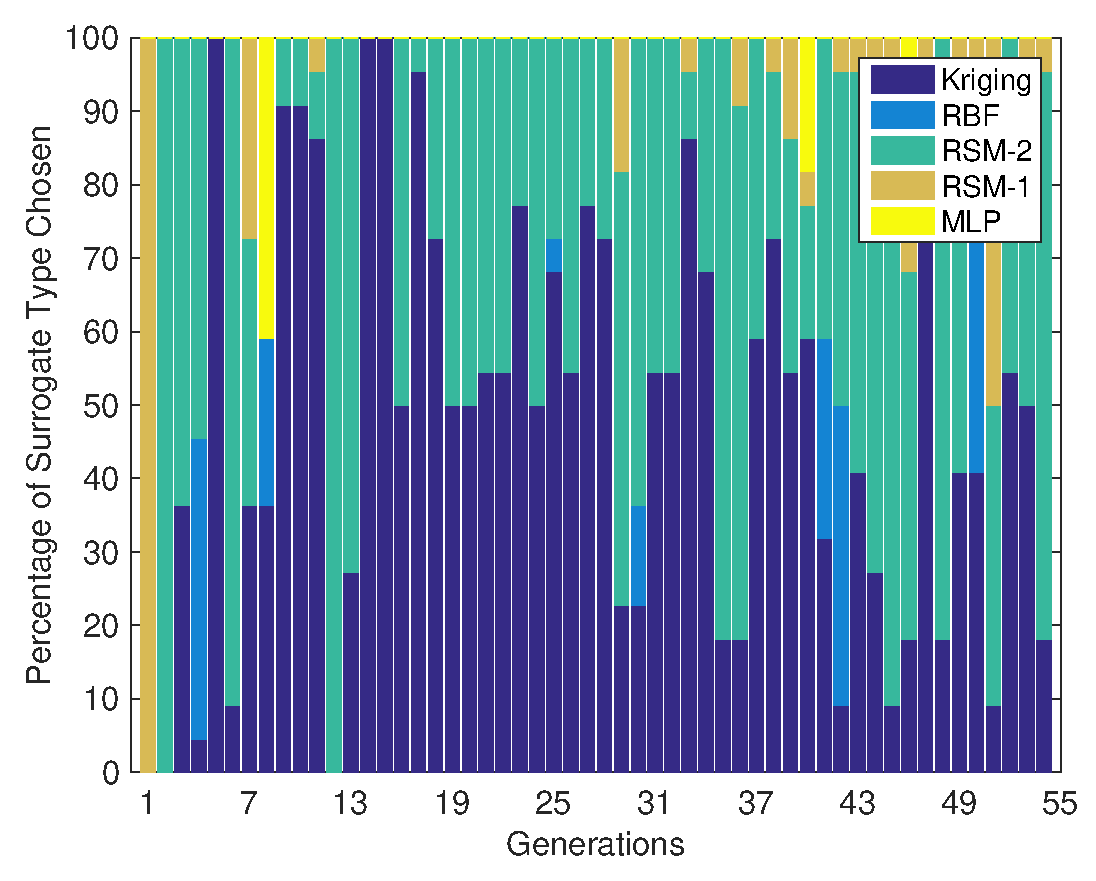
\includegraphics[width=.45\linewidth]{Figures/zdt1_obj2.eps}}
	\caption{Type of surrogate chosen for ZDT1 over generations: (a) First objective (b) Second objective}
	\label{fig:zdt1_type} \end{figure}    

\section{Summary} \label{sec:conclusion} In this paper, we present an algorithm~(SAMO) for the
solution of unconstrained and constrained, multiobjective optimization problems involving
computationally expensive analysis. SAMO relies on NSGA-II~\cite{deb2002fae} as its baseline EA.
However, instead of evaluating the potential offspring solutions directly~(as NSGA-II), a surrogate
assisted evolutionary search is conducted in the neighborhood of every offspring solution using the
best local surrogate model~(Kriging, Radial basis function~(RBF), Polynomial response surface
method~(RSM) of order 1 and 2 and Multilayer perceptrons~(MLP)). The use of \textit{local} surrogate
models for each objective and constraint function offer greater flexibility of representation, while
the choice of the \textit{best} model eliminates the need for complex surrogate fusion/ensemble
strategies. Two mechanisms are examined and compared to pre-select candidate solutions identified
using surrogate assisted neighborhood search for evaluation using actual simulations.

The performance of the proposed approach is studied using a number of well studied numerical
benchmarks and engineering design optimization problems. The benefits of using local best surrogate
models over global best surrogate models have been established. The benefits of improved
pre-selection i.e. pre-selecting offspring solutions with the knowledge of existing parents have also been demonstrated. 
The results clearly indicate the SAMO-IS~(local surrogates with improved pre-selection) offers the best performance
across the problems studied in the paper. The proposed approach can be readily used in conjunction with other
forms of population based stochastic algorithms. The authors are currently exploring the use of such surrogate assisted
schemes for the solution of computationally expensive optimization problems involving 
many objectives~(more than four).

\section{Summary and Future Directions}
\label{sec:sum}


\section{Conclusion}
\label{sec:conc}


\small
